%%% Local Variables: 
%%% coding: utf-8
%%% mode: latex
%%% TeX-engine: xetex
%%% End: 

\pdfinclusionerrorlevel=1
\pdfminorversion=7


\documentclass[aspectratio=169,hide notes,intlimits]{beamer}
\mode<presentation>
{
  \usetheme[footline]{PISMshade}
  \setbeamercovered{transparent}
}

% load packages
\usepackage[english]{babel}
\usepackage[multidot]{grffile}

\usepackage{tikz}
\usetikzlibrary{shadows}

\graphicspath{{figures/}{../2022_04_igs/figures/}{../figures/}{../figures_2018_08/}{../2021_09_cph/figures/}{../2021_11_geo/figures/}}


\newcommand{\mathtext}[1]{\mathsf{#1}}

% title page
\title[Ice sheet modeling] % (optional, use only with long paper titles)
{Calibrated Mass Loss Projections from the Greenland Ice Sheet}
\author[Aschwanden] % (optional, use only with lots of authors)
{\textbf{Andy Aschwanden \& Doug Brinkerhoff}}
\institute{Geophysical Institute, University of Alaska Fairbanks\\
Dept Computer Science, University of Montana, Missoula}

% - Give the names in the same order as the appear in the paper.
% - Use the \inst{?} command only if the authors have different
%   affiliation.

% - Use the \inst command only if there are several affiliations.
% - Keep it simple, no one is interested in your street address.
\titlegraphic{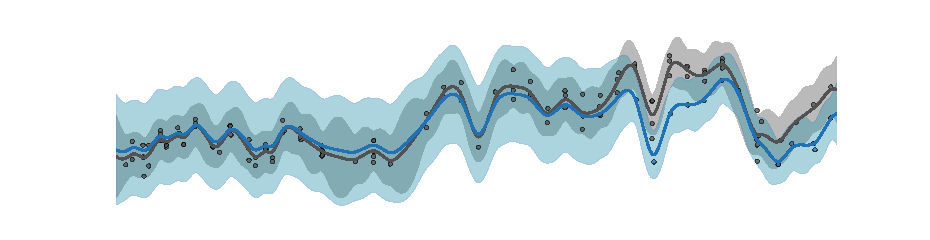
\includegraphics[height=2.5cm]{jib_temperature_forcing_1980_2020_green}\\[.25em]\includegraphics[height=1.cm]{GI_logo_color}\hskip2em
\includegraphics[height=1.cm]{iHARP-Logo_Transparent}\hskip2em
\includegraphics[height=1.cm]{NSF_logo_color}\hskip2em
\includegraphics[height=1.cm]{nasa-logo}\hskip2em
\includegraphics[height=.75cm]{university_of_montana_logo}}

\date{}


\subject{Credible sea-level projections}

\begin{document}


\setbeamertemplate{background canvas}
  {
     \tikz{\node[inner sep=0pt,opacity=1.0] {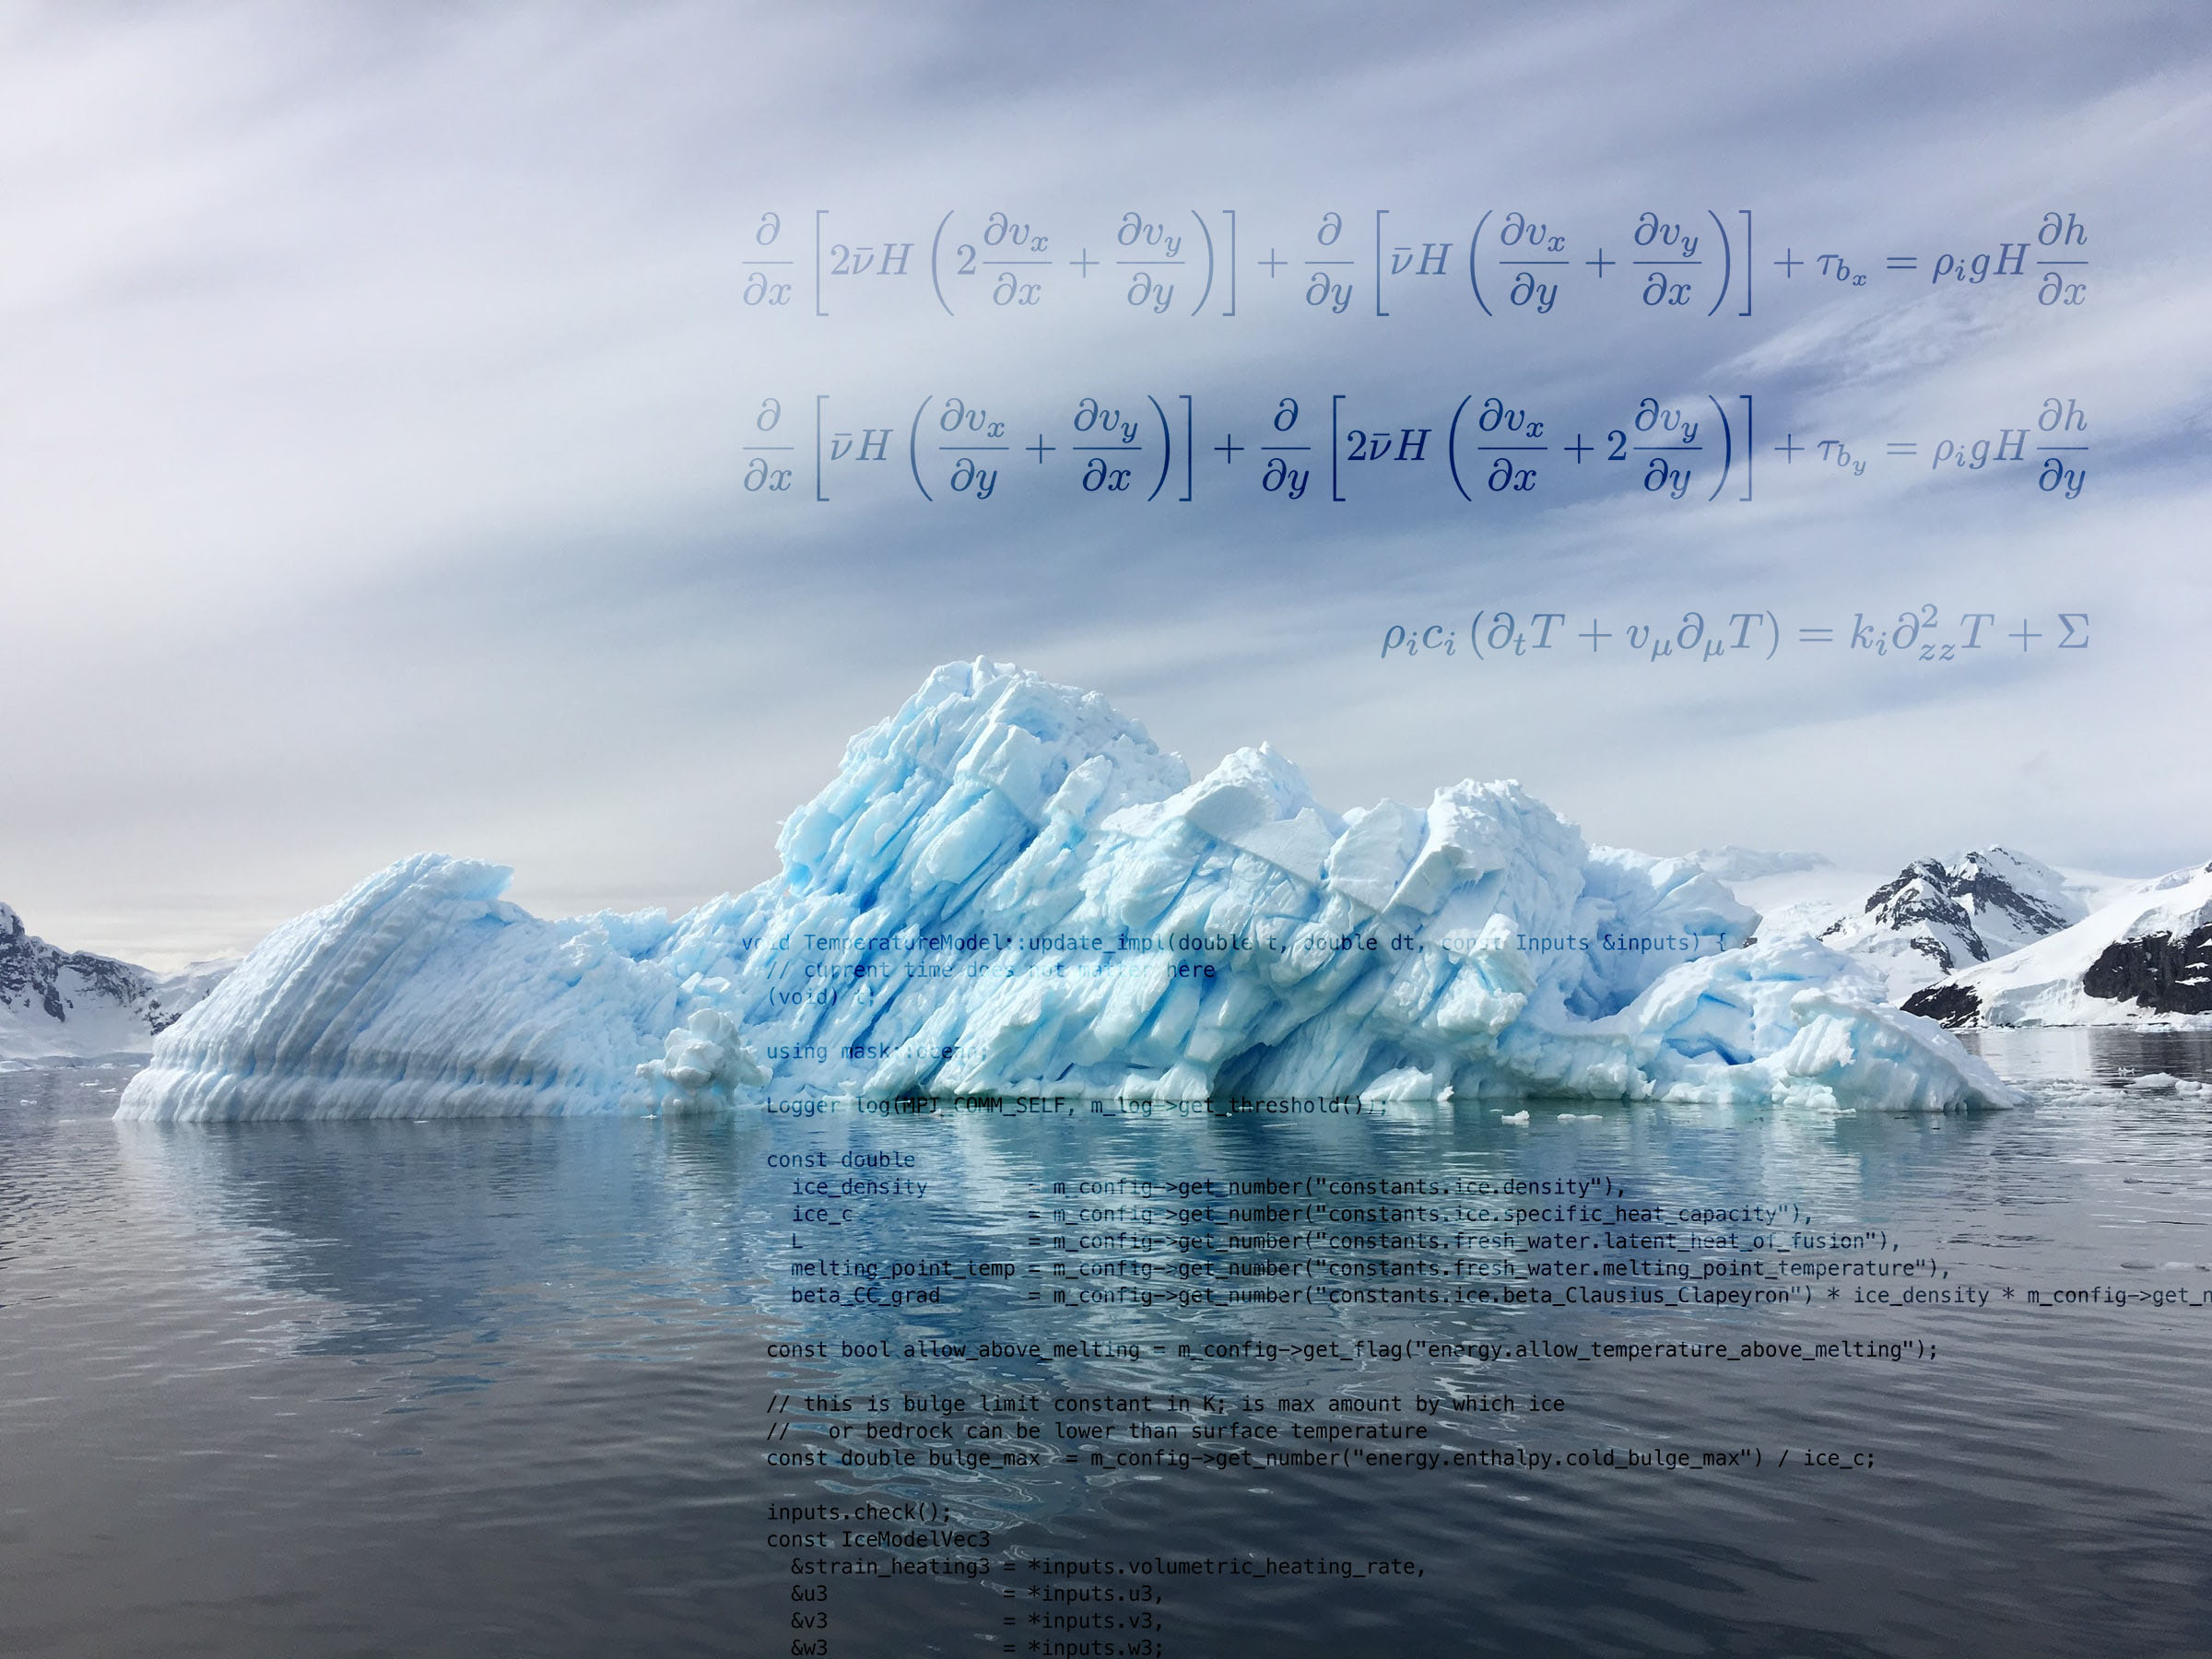
\includegraphics[width=\paperwidth]{header_ice_equations}};}

  }

\plainframe{}


  \setbeamertemplate{background canvas}
  {
}

  
\begin{frame}[noframenumbering]
    \begin{minipage}[t][5.25cm][t]{\textwidth}
  \begin{figure}
    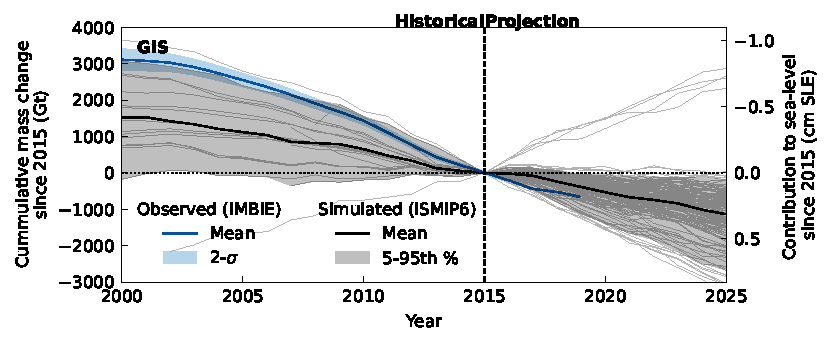
\includegraphics[width=.75\textwidth]{GIS_historical}\\[-1em]
    {\tiny{Aschwanden, Brinkerhoff, Bartholomaus \& Truffer (2021)}}
  \end{figure}
    \end{minipage}
    \begin{minipage}[t][3.5cm][t]{\textwidth}
    \textbf{Uncertainties} due to
        \begin{columns}[c]
    \begin{column}{.18\textwidth}
\begin{itemize}\setlength\itemsep{.25em}
    \item \alert{Parameters}
    \item Models
\end{itemize}
    \end{column}
    \begin{column}{.4\textwidth}
\begin{itemize}\setlength\itemsep{.25em}
    \item Forcing
    \item Initial State (Poster by A. Pohle, C51D-0982)
\end{itemize}
    \end{column}
    \begin{column}{.25\textwidth}
    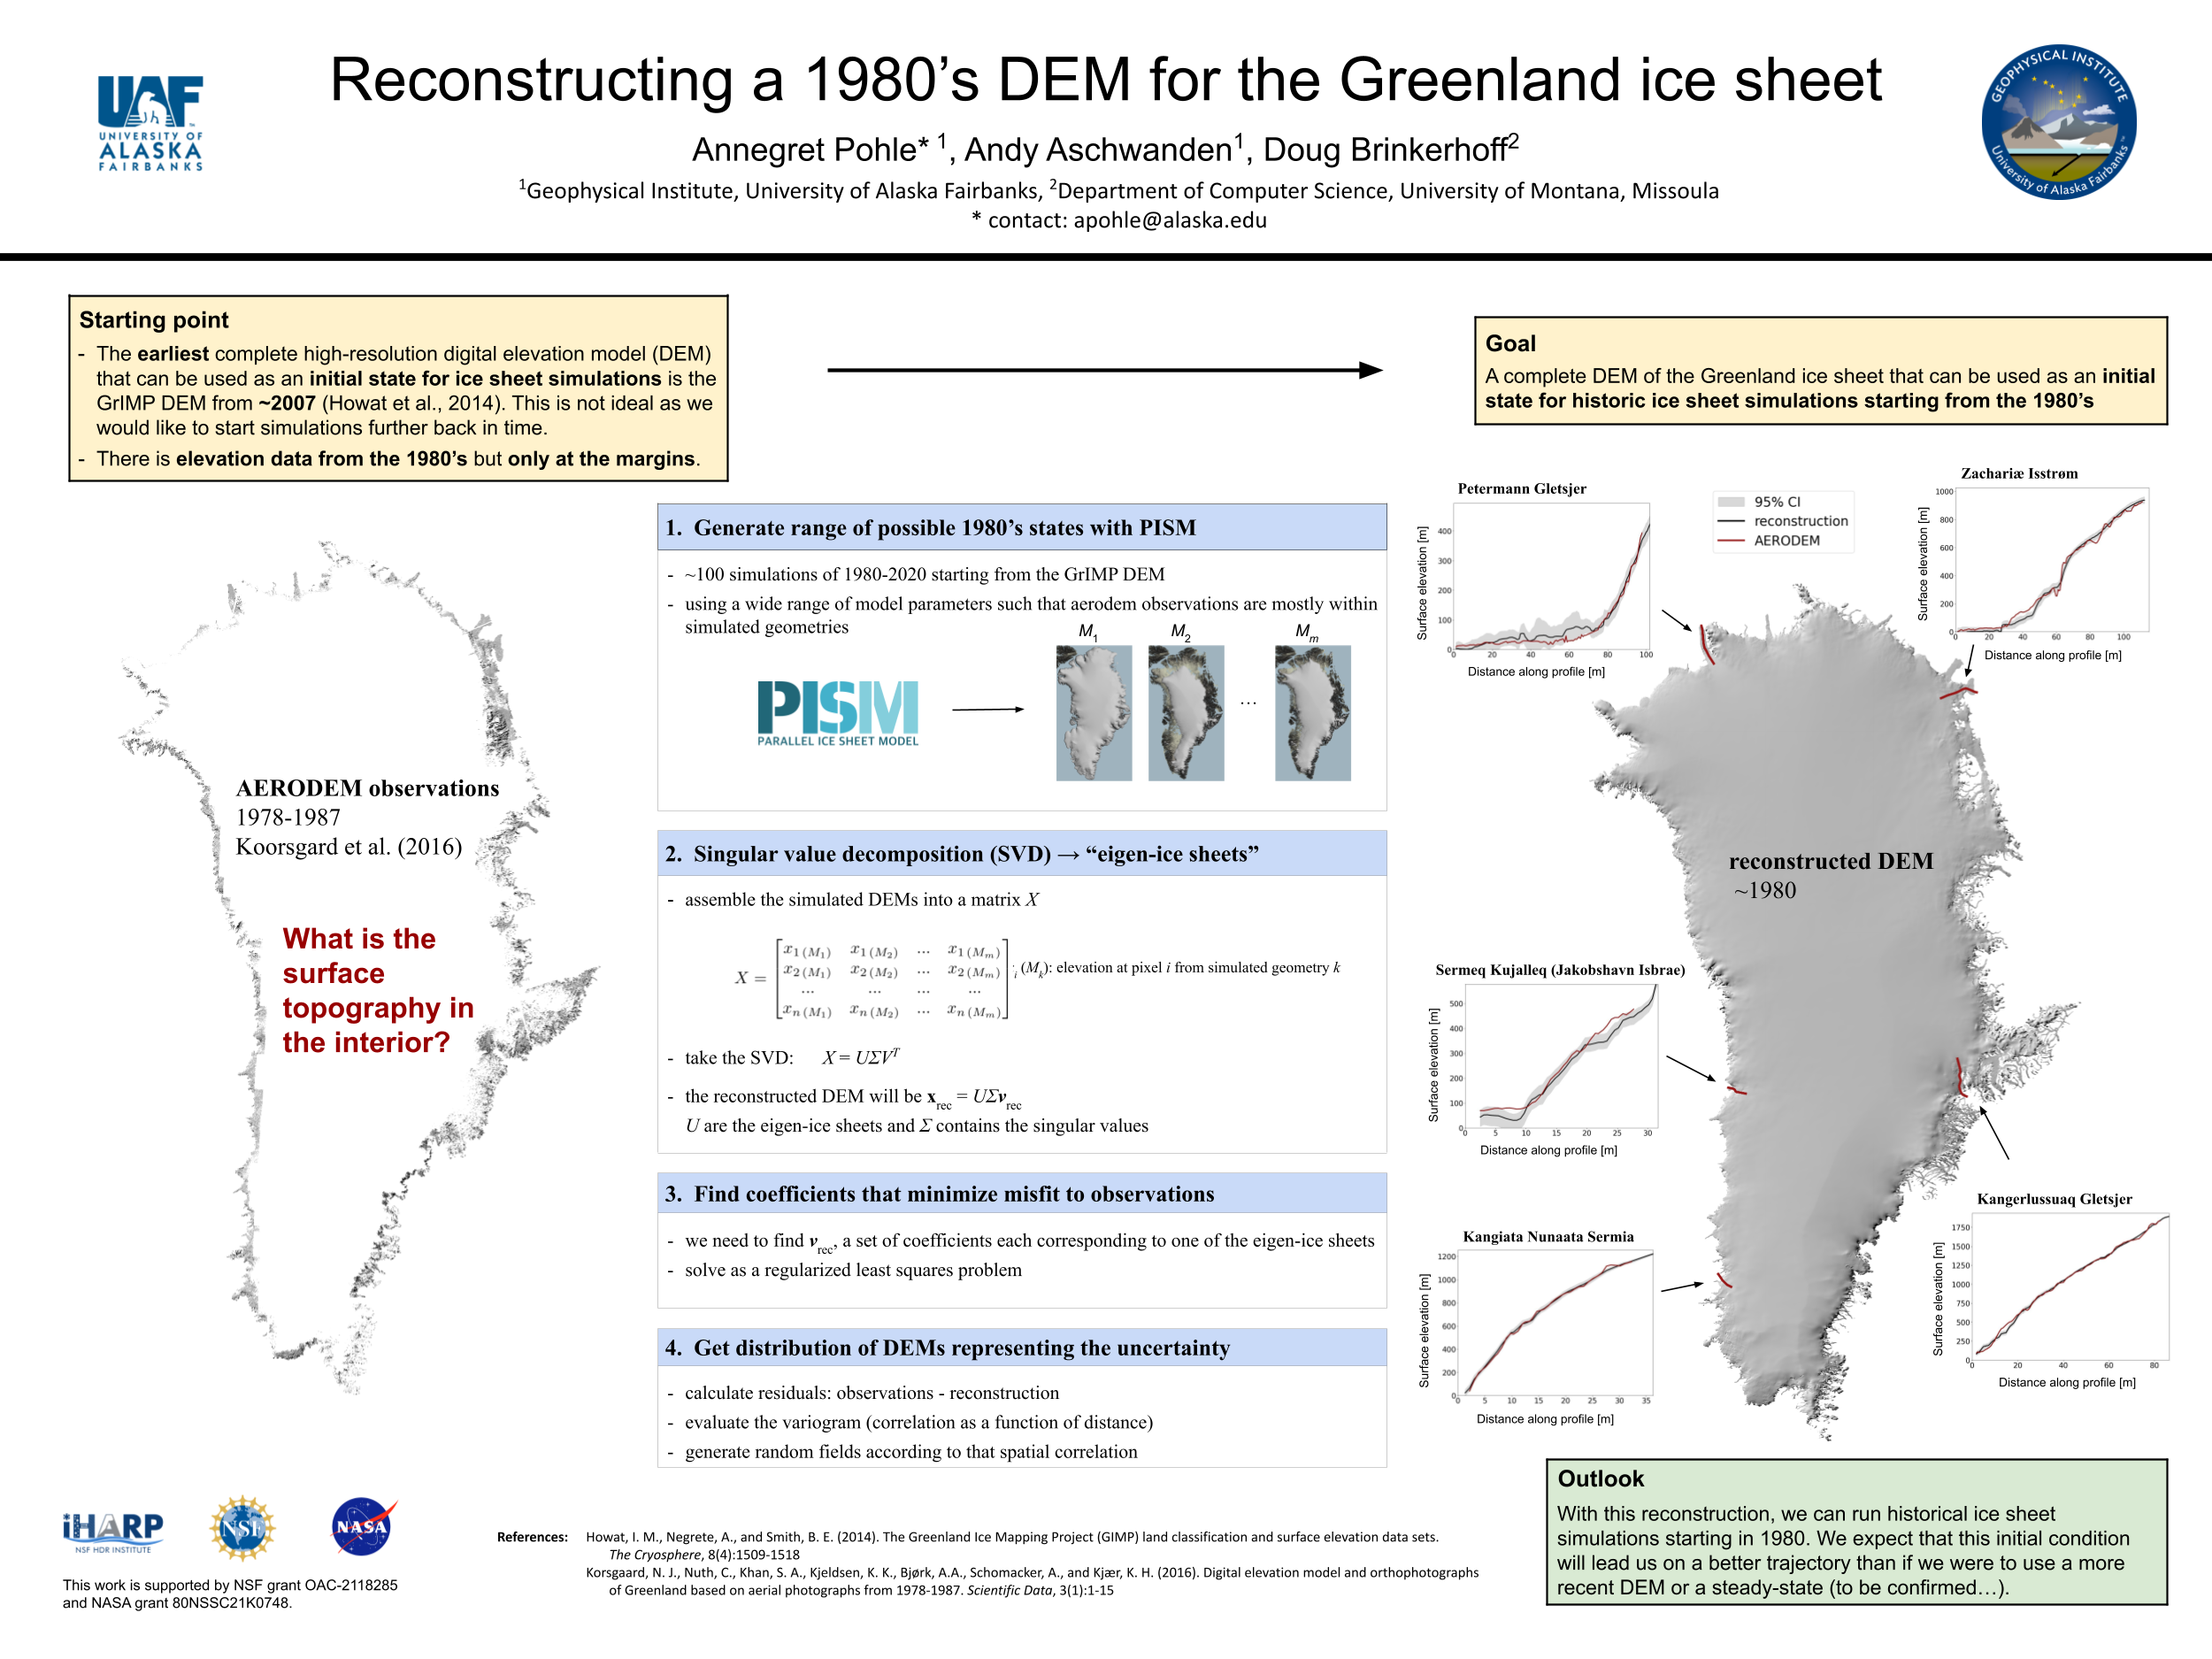
\includegraphics[width=.75\textwidth]{pohle_poster_agu_2023}    
    \end{column}
  \end{columns}
    \end{minipage}
\end{frame}


% insert titlepage
\begin{frame}
  \titlepage
\end{frame}

\setbeamertemplate{background canvas}
  {
}


\begin{frame}{2-step Probabilistic Calibration}
  \begin{figure}
    \includegraphics<1>[width=10cm]{slr-probability}    
  \end{figure}
\begin{equation*}
P\left(\Delta_{2100} | \mathbf{D}, \mathcal{H}, \mathcal{F} \right)
 = \int \underbrace{P\left(\Delta_{2100} | \mathbf{M},\mathcal{H}, \mathcal{F} \right)}_{\text{Projection}} \alert{\underbrace{P\left(\mathbf{M} | \mathbf{D},\mathcal{H}, \mathcal{F} \right)}_{\text{Calibration}}}\, \mathrm{d} \mathbf{M},
\end{equation*}
\begin{enumerate}
\item Calibration of model parameters
\item Particle filtering (aka importance sampling, Bayesian calibration)
\end{enumerate}
\end{frame}

\begin{frame}{Which observations should we use?}
    \begin{minipage}[t][1.2cm][t]{\textwidth}
        \begin{itemize}
        \item use the quantity of interest: \alert{mass change}
        \item use quantity that contributes a lot to uncertainty: \alert{ice flow}
        \end{itemize}
  \end{minipage}
    \begin{minipage}[t][10cm][t]{\textwidth}
        \begin{columns}[c]
    \begin{column}{.3\textwidth}
   \begin{block}{Surface Speeds}
    \includegraphics[height=5cm]{greenland-obs-rignot}
    \end{block}
    \end{column}
    \begin{column}{.65\textwidth}
   \begin{block}{Mass Change}
    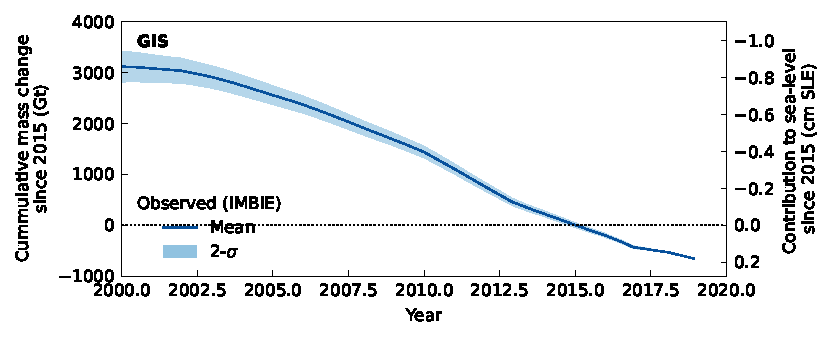
\includegraphics[height=4cm]{GIS_hist_only_obs}
    \end{block}
    \end{column}
  \end{columns}
    \end{minipage}
\end{frame}



\begin{frame}{}
  \vspace{-1.5em}
    \begin{minipage}[t][8.2cm][t]{\textwidth}
    \begin{figure}
      \includegraphics[height=8cm]{surrogate_model_all_pism}
    \end{figure}
    \end{minipage}
\end{frame}


\begin{frame}{Uncalibrated Simulations}
\begin{columns}[c]
    \begin{column}{.5\textwidth}
      \begin{figure}
        \includegraphics<1>[height=7.5cm]{sle_pdf_w_obs_as19_2020.pdf}
    \end{figure}
    \end{column}
    \begin{column}{.5\textwidth}
    \end{column}
  \end{columns}

\end{frame}


\begin{frame}{Flow Calibration}
\begin{columns}[c]
    \begin{column}{.5\textwidth}
      \begin{figure}
        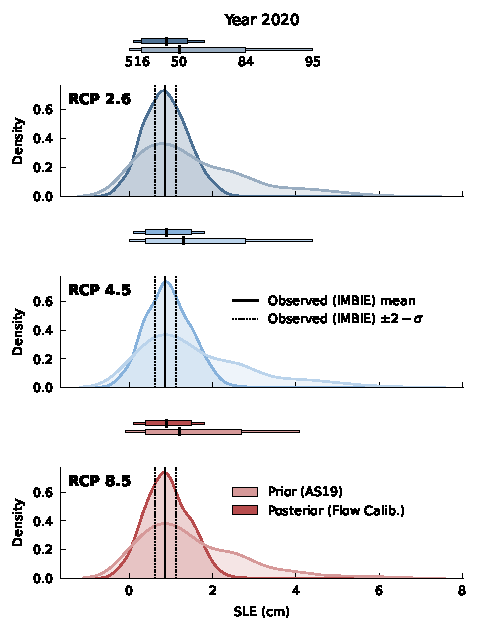
\includegraphics[height=7.5cm]{sle_pdf_w_obs_as19flow_2020.pdf}
    \end{figure}
    \end{column}
    \begin{column}{.5\textwidth}
      \begin{figure}
    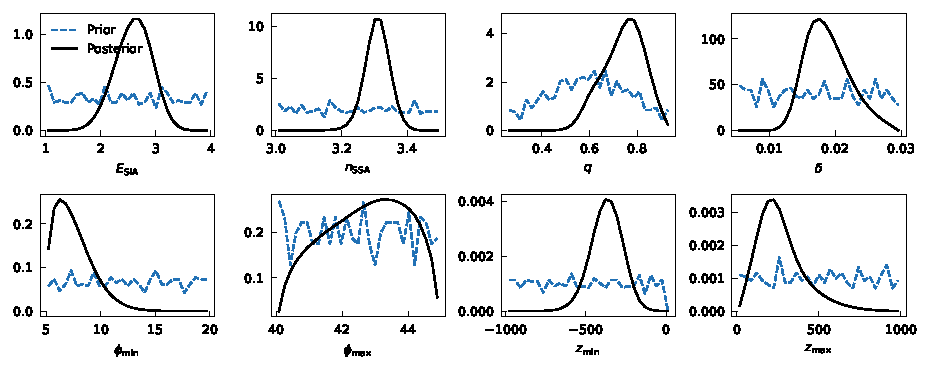
\includegraphics[width=0.85\textwidth]{prior_posterior}
  \end{figure}

  \begin{itemize}
  \item<1> create 500 samples from posterior
  \item<1> rerun PISM 500x, wait
  \item<2> get new projections conditioned on surface speeds
  \item<2> find reduced variance
  \end{itemize}
    \end{column}
  \end{columns}

\end{frame}


\begin{frame}{2. Mass Loss: Particle Filtering}
  \begin{equation*}
    \label{eq:parameter_posterior}
    P(\mathbf{M}|\mathbf{u}_{\mathrm{obs}},\Delta_{\mathrm{obs}}) \propto P(\Delta_{\mathrm{obs}}|\mathbf{M}) P(\mathbf{m}^{*}) P(\mathbf{m}_{\mathrm{flow}}|\mathbf{u}_{\mathrm{obs}})
  \end{equation*}
  \begin{minipage}[t][4cm][t]{\textwidth}
    \begin{figure}
    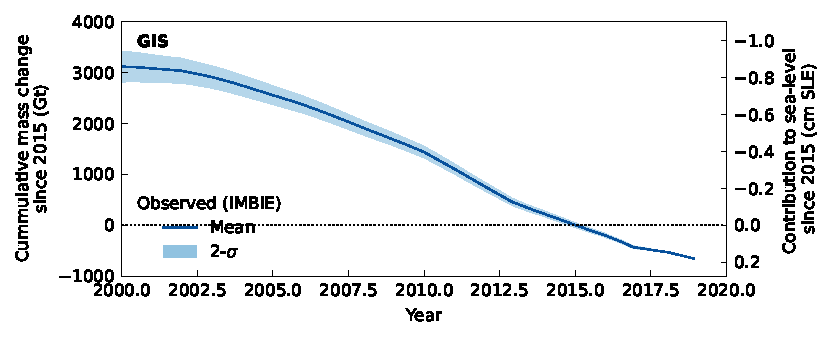
\includegraphics[height=3.5cm]{GIS_hist_only_obs}
    \end{figure}
  \end{minipage}
  \begin{itemize}
  \item  weight members based on their likelihood relative to observations of mass change.
  \item resample simulations proportionally to these likelihoods to create a new ensemble that is consistent with respect to both  observations of surface speed and mass change to within observational uncertainty
  \end{itemize}
\end{frame}


\begin{frame}{Posterior distributions}
  \begin{columns}[c]
    \begin{column}{.5\textwidth}
      \begin{figure}
        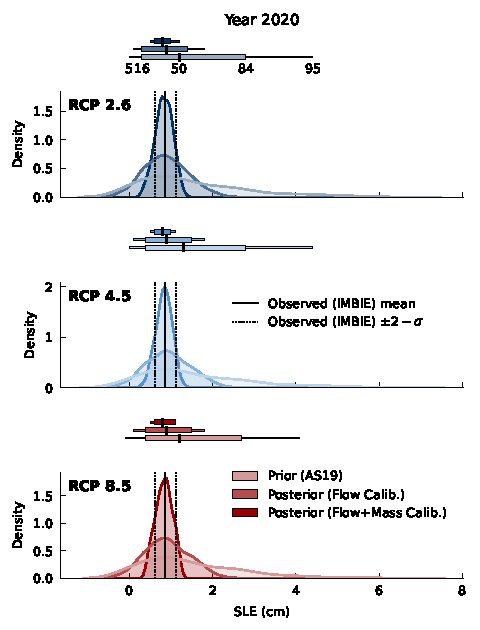
\includegraphics[height=7.75cm]{sle_pdf_w_obs_calibrated_2020.pdf}
      \end{figure}
    \end{column}
    \begin{column}{.5\textwidth}
      \begin{itemize}
      \item fully calibrated posterior agrees well with observations (IMBIE)
      \item (which is by design)
      \end{itemize}
    \end{column}
  \end{columns}
\end{frame}



\begin{frame}{Calibrated 2100 Projections}
    \begin{figure}
      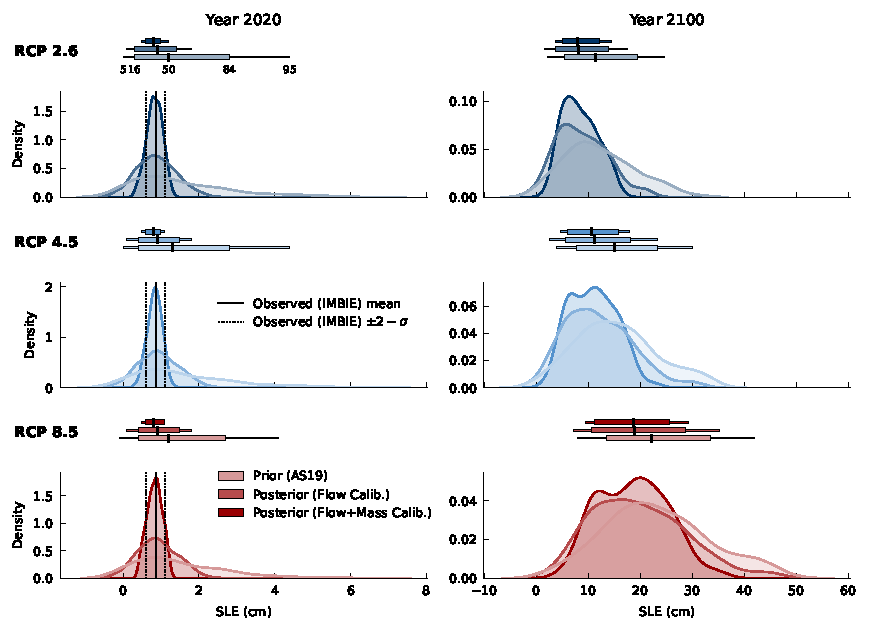
\includegraphics[height=7.75cm]{sle_pdf_w_obs_2020_2100}
    \end{figure}
\end{frame}



\end{document}
